% A2 — ICASSP 2027 paper spec (execution-methodology Step 1).
% Scope guard: an experiment runs only if it fills a cell of this paper.
% Claim margins (Step 4), all below pilot-observed values:
%   pinned FPR within +-2pp at N>=100 (pilot EXP-002: exactly 5.0% at N>=100);
%   FNR within 2 pts of oracle on usable cells (pilot: <=0.7 pts at N=500);
%   matched-resource cohort norm off by >2pp on the majority of cells
%   (pilot EXP-010: 6/8 cells for z-norm, 8/8 for robust).
% The drift map is complete; the numerical claims below are bound to results_drift.json.
% 2026-09-09: every ASVspoof 2021 number excludes the hidden (VAD-trimmed) phase;
% see experiments/EXP-102-a2-campaign/AMENDMENT-3-trial-phase-protocol.md.
\documentclass{article}
\usepackage{spconf,amsmath,graphicx,booktabs,tabularx,url}

% Retitled on external review (Phase 9). The criterion framing is retired
% STRUCTURALLY, not by a disclaimer: the additive band ranks conservative
% severity at rho=0.9999, so the ratio scale buys a bar and not information.
% The lead is the operational finding; the title names the mechanism and the
% paradox without a fold ratio, which one cell cannot support.
\title{TRANSPORTED ANTI-SPOOFING THRESHOLDS CAN FAIL CONSERVATIVELY: MISSED SPOOFS AT A FALSE-ALARM RATE BELOW TARGET}
%
\name{\shortstack{Rafaello Virgilli, Lucas Alc\^antara Souza, Alexandre Costa Ferro Filho, Daniel Tunnermann,\\
Gustavo dos Reis Oliveira, Arlindo Rodrigues Galv\~ao Filho, and Anderson da Silva Soares}}
\address{Advanced Knowledge Center in Immersive Technologies (AKCIT)\\
Federal University of Goi\'as (UFG), Goi\^ania, GO, Brazil}

% Camera-ready float spacing: the class defaults leave ~13pt above and below
% every float, which at three floats costs more than a text line. These are the
% standard LaTeX float-separation parameters, not a rule change.
\setlength{\textfloatsep}{8pt plus 2pt minus 2pt}
\setlength{\floatsep}{12pt plus 2pt minus 2pt}
\setlength{\intextsep}{8pt plus 2pt minus 2pt}
\setlength{\dbltextfloatsep}{8pt plus 2pt minus 2pt}
% Reference list at zero item separation: the standard list parameters, so the
% bibliography fits the references-only page 5.
\let\spconfthebibliography\thebibliography
\def\thebibliography#1{\spconfthebibliography{#1}\setlength{\itemsep}{0pt}\setlength{\parsep}{0pt}}

\begin{document}
\maketitle

\begin{abstract}
In our tested channel and corpus transfers, speech-deepfake thresholds calibrated to 5\% false-positive rate (FPR, bona fide rejected) often miss that target. Across 108 combinations of two detectors and source--target conditions, 77 realize an FPR more than $2\times$ off target (36 above, 41 below). Over 1,000 random cohorts of 500 recordings drawn from 2,356 PSTN bona-fide trials, AASIST yields mean \textbf{0.42\% FPR} on all 2,356 G.722 bona-fide recordings and misses \textbf{70\%} of its 21,164 spoofs; an oracle threshold on all target bona fide misses \textbf{0.66\%}. On speaker- and recording-disjoint ASVspoof~5 data, 49 of 66 SSL-AASIST transfers to six destinations with oracle FNR $\le$50\% yield mean FPR below 2.5\%. Over all 66 transfers, excess FNR (mean transported FNR minus destination-oracle FNR) has median \textbf{0.8} points from sources with oracle FNR $\le$50\%, 11 of 30 exceeding $+10$, and \textbf{68.8} from sources with oracle FNR $>$50\%. Using 500 target bona-fide recordings, an order statistic restores mean FPR to 4.91--5.06\% across three detectors on four corpora. Its guarantee is marginal under exchangeable sampling; a whole-speaker diagnostic widens FPR spreads for AASIST and SSL-AASIST across three channel conditions. Fixed-threshold deployments should therefore report both error rates, the calibration sampling unit and its dispersion.
\end{abstract}

\begin{keywords}
Anti-spoofing, audio deepfake detection, threshold calibration, conformal prediction, domain shift
\end{keywords}

\section{Introduction}
\label{sec:intro}
% MINIMUM interesting claim (pilot-exceeded, margins in header comment):
%  (i) naive transfer fails catastrophically on the field's standard corpora
%      -- our own measurement, same checkpoints;
% (ii) the bona-fide quantile pins FPR within +-2pp from N=100, FNR cost
%      <=2 pts of oracle on viable corpora (ITW decisive);
% (iii) the same N labels spent on cohort normalization do NOT control FPR
%      (majority of cells off by >2pp) -- the win is distribution-freeness,
%      not labels;
%  (iv) failure regimes are characterized honestly (BRSpeech overlap cell;
%      drift map measured, outcome not pre-claimed).

Anti-spoofing studies usually report equal error rate (EER), measured at an oracle threshold selected with labels from both classes; a deployed service must fix a threshold in advance and accept the resulting false-positive rate.  A threshold set to 5\% FPR on ASVspoof~2019~LA dev \cite{asvspoof19} realizes 22--98.5\% FPR across 21LA/21DF \cite{asvspoof21}, In-the-Wild \cite{itw}, and BRSpeech-DF \cite{brspeechdf} for a strong open-source detector \cite{tak22}. Transfer failures of this kind are documented in \cite{eerhides26,kwok25}, and presentation can matter more than model scale \cite{delgado26}. LRLspoof \cite{lrlspoof26} transfers an EER threshold across 66 languages without target bona fide and can report only spoof rejection; we assume the converse resource and evaluate the FPR side.

We study the deployment behavior of a standard statistical repair: given $N$ labeled target-domain \emph{bona-fide} recordings and no spoof labels, the $\lfloor(N{+}1)\alpha\rfloor$-th order statistic has marginal rank validity under exchangeability without ties, and under iid continuous sampling its conditional FPR follows an exact finite-sample Beta law \cite{tong18,vovk}; conservative Neyman--Pearson variants give high-probability upper bounds \cite{tong18}. Neither the statistic nor bona-fide-only audio calibration is new \cite{zhao26ca}. Our contribution is empirical: we measure transport across channels and corpora, its spoof-side cost, its persistence on disjoint data, and what alternative policies buy at the same labeling budget.

\section{Related work}
\label{sec:related}
% Provenance-first paragraph (Gate-2 evidence): the method is old, cite it as such.
Order-statistic calibration is established: Neyman--Pearson methods control type-I error through class-0 order statistics \cite{tong18} and negative-only conformal calibration provides marginal guarantees \cite{vovk}. Zhao et al.\ use a bona-fide-only $\alpha$-quantile \cite{zhao26ca}; \cite{kwok25} reports bona-fide cross-testing errors. Zhou and Wang \cite{eerhides26} transfer a source EER threshold (ITW: 78.7\% bona fide rejected). We quantify recoverable spoof misses against a destination oracle at fixed source FPR, using a 108-cell channel/corpus map with real transmissions, finite-$N$ target-bona-fide calibration and a 264-pair disjoint replication. Auditing both error rates at a preset threshold is established in spoofing evaluation \cite{asvspoof5}, and \cite{rubio26} holds a cost-optimal threshold fixed across the same 21LA codecs but reports relative cost only. Khan et al.'s TRACE \cite{trace26} contrasts transferred and target-selected thresholds for partial deepfakes. Demographic threshold calibration \cite{fursule26} likewise separates class-conditional error changes from unchanged discrimination. ReplayDF \cite{muller25replay} reports channel-induced spoof-side degradation with stable bona-fide acceptance. Sch\"afer and Steinebach \cite{schaefer26} evaluate detectors on social-media audio at preset thresholds and find transferred thresholds that admit more spoofs while accepting more bona fide; we measure that cost against a destination oracle at a fixed bona-fide error target.



Ramos et al.\ \cite{ramos26} analyse the calibration-conditional Beta law under dependence, where we add an empirical speaker-level diagnostic. % Scoop re-run 2026-08-14: ICASSP 2026 swept (4,589-paper Crossref TOC + 795 abstracts)
% and Odyssey 2026 -- zero conformal/FPR-band/operating-point papers in audio; clear.
% Interspeech 2026 sweep closed 2026-08-28: all 1,416 rows (1,384 numbered papers) in
% the official program were screened; 77 title/session hits and the closest available
% preprints were read. No competing fixed-FPR, target-bona-fide calibration study was
% found. LRLspoof is the one threshold-transport neighbor and is cited above. Audit log:
% PRIOR-ART-SWEEP-INTERSPEECH-2026.md.

\section{Threshold policies}
\label{sec:method}
We treat spoof as the positive class. A detector emits score $s$ (higher = bona fide), and deployment flags spoof when $s<t$, so $\mathrm{FPR}(t)=\Pr(s<t\mid\text{bona fide})$ is the bona-fide rejection rate ($P^{\mathrm{cm}}_{\mathrm{miss}}$ in the ASVspoof convention) and $\mathrm{FNR}(t)=\Pr(s\ge t\mid\text{spoof})$ the spoof acceptance rate. ``Calibration'' below means selecting $t$ for a target FPR, not probability calibration. We compare policies by resource class. With \textbf{no target data}, the source dev threshold $t$ at the target FPR is transferred unchanged. With \textbf{unlabeled target data}, we fit variants of the corrections of \cite{eerhides26}: each transform is fitted to the unlabeled source and target mixtures separately, the 5\% quantile of transformed source bona fide is taken, and that threshold is applied to transformed target scores. C1 is z-norm. With \textbf{$N$ labeled target bona-fide recordings}, we test three policies: (a) cohort z-norm sets $t=\bar s_N+\hat\sigma_N\,(t_{\mathrm{src}}-\mu_{\mathrm{dev}})/\sigma_{\mathrm{dev}}$, with $t_{\mathrm{src}}$ the 5\% quantile and $\mu_{\mathrm{dev}},\sigma_{\mathrm{dev}}$ the mean and standard deviation of the source-development bona fide ($\hat\sigma_N^2=N^{-1}\sum_i(s_i-\bar s_N)^2$, and $\sigma_{\mathrm{dev}}$ uses the same divisor); (b) the Gaussian parametric quantile sets $t=\bar s_N - 1.645\,\hat\sigma_N$; and (c) the \emph{conformal quantile} sets $t$ to the $k$-th smallest cohort score, where $k=\lfloor(N{+}1)\alpha\rfloor$. Exchangeability without ties gives the last policy's marginal rank guarantee. Under iid continuous sampling from a fixed score distribution, its conditional FPR across calibration draws additionally follows $\mathrm{Beta}(k, N{+}1{-}k)$ \cite{tong18,vovk}. The \textbf{target-bona-fide oracle} sets $t$ to the empirical $\alpha$-quantile of all deployment bona-fide scores; spoof labels measure its FNR but do not select it.
\textbf{Definitions.} A detector--corpus cell is \emph{overlap-dominated} when its oracle FNR at the target FPR exceeds 50\%: it has no usable operating point under our joint criterion, is italicised in Table~\ref{tab:fnr}, and is excluded from claims about usable cells. The Beta dispersion is an iid-continuous population reference, not the law of finite-pool draws without replacement; we report the empirical spread separately. C4 (CORAL) of \cite{eerhides26} additionally requires applying the frozen classifier head to transformed embeddings and is not evaluated.

\section{Experiments}
\begin{table}[!tp]
\caption{EER and conformal errors (\%); 21LA pools seven conditions. EER uses each system's full retained evaluation pool; conformal FPR uses the bona-fide complement of each calibration cohort and FNR the retained spoof pool, and official XLS-R+SLS 21DF scores include five spoof trials excluded for the other two. Conformal means use $B{=}1000$ paired $N{=}500$ cohorts targeting FPR${=}5\%$; parentheses give mean FNR minus deployment-oracle FNR (points). Per-condition 21LA EER ranges: 1.9--11.1 (AASIST), 0.2--1.0 (SSL-AASIST), 0.5--3.5 (XLS-R+SLS). Within a policy, FPR and FNR share thresholds; labeled-policy means come from separate runs and are not paired across policies. Naive transfer and C1 are deterministic. Italics: oracle FNR ${>}50\%$, no usable operating point. Scores, code and results: \protect\url{https://github.com/rvirgilli/speech-deepfake-threshold-transport/tree/a2-icassp2027-final}.}
\label{tab:fnr}
\centering\small\setlength{\tabcolsep}{0.8pt}
\begin{tabular}{lcccc}
\toprule
System & 21LA & 21DF & ITW & BRSpeech \\
\midrule
\multicolumn{5}{l}{\emph{Pooled EER (\%)}} \\
AASIST & 8.26 & 14.16 & 43.02 & 36.06 \\
SSL-AASIST & 0.81 & 5.86 & 11.20 & 34.69 \\
XLS-R+SLS$^\dagger$ & 2.80 & 1.98 & 7.46 & 34.17 \\
\midrule
\multicolumn{5}{l}{\emph{Conformal FNR (\%) and oracle difference (pp)}} \\
AASIST & 19.1 (+0.4) & 36.7 (+0.1) & \emph{95.1 ($-$0.1)} & \emph{84.0 ($-$0.3)} \\
SSL-AASIST & 0.2 (+0.0) & 6.9 (+0.1) & 18.3 (+0.2) & \emph{98.5 (0.0)} \\
XLS-R+SLS$^\dagger$ & 1.5 (+0.1) & 0.7 (+0.1) & 11.3 (+0.5) & \emph{91.5 (+0.4)} \\
\midrule
\multicolumn{5}{l}{\emph{Realized FPR (\%) at the conformal quantile, same run}} \\
AASIST & 5.06 & 5.04 & 5.02 & 5.01 \\
SSL-AASIST & 4.95 & 5.00 & 4.99 & 4.93 \\
XLS-R+SLS$^\dagger$ & 4.97 & 4.91 & 4.93 & 4.98 \\
\midrule
\multicolumn{5}{l}{\emph{SSL-AASIST policies: FPR/FNR (\%)}} \\
Naive transfer & 22.2/0.06 & 38.4/0.02 & 98.5/0.08 & 95.7/1.18 \\
C1 z-norm & 18.7/0.08 & 24.5/0.32 & 100.0/0.00 & 100.0/0.06 \\
Cohort z-norm & 7.4/0.2 & 20.3/0.9 & 11.9/10.7 & 23.2/73.1 \\
Gaussian q. & 5.6/0.2 & 11.9/2.8 & 5.7/17.2 & 0.0/100.0 \\
\bottomrule
\end{tabular}\\[2pt]
{\small $^\dagger$Official author-released scores for 21LA, 21DF and ITW; BRSpeech scored by us with the released checkpoint.}
\end{table}
\begin{table}[!tp]
\centering
\caption{Transport settings behind the title. Thresholds target 5\% source FPR; excess
FNR is mean transported FNR minus destination-oracle FNR. The A5 rows are SSL-AASIST's 66
transfers to the six destinations with oracle FNR ${\le}50\%$, split on whether the
calibration condition is itself usable (weak = overlap-dominated); medians cover every
cell mean, not only the conservative misses, and 11 of the 30 usable-source transfers
still exceed $+10$. Cells are dependent.}
\label{tab:settings}
\begin{tabularx}{\columnwidth}{@{}XXX@{}}
\hline
Setting & FPR ${<}2.5\%$ & Excess FNR (pts) \\
\hline
AASIST 21LA PSTN$\to$G.722 & 0.42\%, one cell & $+69.4$ \\
A5 usable source & 15/30 & $+0.8$ median \\
A5 weak source & 34/36 & $+68.8$ median \\
\hline
\end{tabularx}
\end{table}
\begin{figure}[!tp]
\centering
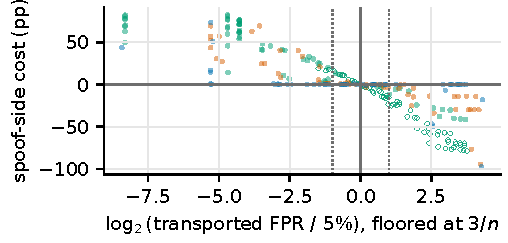
\includegraphics[width=\columnwidth]{figs/drift.pdf}
% REWRITTEN 2026-08-14 after the Gate-8 correctness audit. The previous caption
% plotted and quoted |FPR-5%|, which saturates at 5 pp on the conservative side,
% and attributed a Spearman of 0.64 to this panel -- that number is the cell-9
% mixture-$W_1$ monitor's, not this panel's oracle-$W_1$ statistic. Counts below
% depend on post-hoc bars and are reported as such; see the EXP-102 addendum.
\caption{Transported FPR against spoof-side cost. Each point is one deployment cell: severity $\log_2(\max(\mathrm{FPR},3/n)/5\%)$ (\S4; dotted lines mark the $2\times$ bar) against mean FNR at the transported threshold minus FNR at the all-target-bona-fide oracle threshold, in points. Blue circles (SSL-AASIST) and orange squares (AASIST) show the 108 21LA and cross-corpus cells; green triangles show the 132 ASVspoof~5 SSL-AASIST pairs, filled where the destination is usable (oracle FNR $\le$50\% for every source) and hollow where it is overlap-dominated.}
\label{fig:drift}
\end{figure}
\label{sec:exp}
\textbf{Setup.} We evaluate AASIST \cite{jung22}, SSL-AASIST \cite{tak22}, and XLS-R+SLS \cite{zhang24sls}. The first two use released 19LA-trained checkpoints. XLS-R+SLS score provenance is specified in Table~\ref{tab:fnr}. The corpora are ASVspoof 2021 LA and DF \cite{asvspoof21}, In-the-Wild \cite{itw}, BRSpeech-DF \cite{brspeechdf} (6,587 test spoofs from its release; 1,320 bona fide from the separate CML-TTS release \cite{cmltts23}; all cml/ filenames match the BRSpeech-DF test roster without establishing waveform identity; class and release are confounded, so results describe this release pairing), and ASVspoof~5 eval \cite{asvspoof5} for replication. The 2021 keys carry \emph{eval}, \emph{progress} and \emph{hidden} phases; the hidden phase removes non-speech by voice-activity detection and was not used in challenge results \cite{asvspoof21taslp}. Non-speech is a documented shortcut for these detectors \cite{rubio26}, so the trimmed subset is a shortcut-removed benchmark \cite{dao26} rather than a deployment channel, and mixing it into a calibration cohort mixes two score populations. A first version of this study did so; as a post-hoc protocol correction, every result below excludes it and keeps the two untrimmed phases, and restricting to the eval phase alone preserves every grid total below while trial counts and individual rates change. Each 21LA condition is then the same 2,356 bona-fide recordings of 67 speakers and 21,164 spoofs: six conditions are real transmissions, five through an Asterisk PBX over VoIP and one over a PSTN carrier, and one is the untransmitted source \cite{asvspoof21}. Every detector is evaluated on the full 21LA and 21DF sets (16,492 and 20,637 bona fide; five 21DF spoof files were undecodable for our two detectors and excluded). For cross-corpus transport the 21LA node is its untransmitted condition only (2,356 bona-fide and 21,164 spoof trials); Table~\ref{tab:fnr} instead pools all seven conditions. All thresholds target $\alpha{=}5\%$. Within each Monte Carlo run, labeled policies share paired cohort draws ($B{=}1000$); Table~\ref{tab:fnr} combines unpaired means from separate runs. FPR is measured on held-out data.

\textbf{FPR control and FNR cost.} At $N{=}500$, the conformal quantile's mean realized FPR is 4.91--5.06\% across the 12 detector--corpus cells (Table~\ref{tab:fnr}), and in a separate 1000-draw diagnostic on the same score sets the 2.5--97.5 percentile spread of realized FPR lies within 2.8--7.6\% on every cell, close to the iid Beta reference. On every cell with a usable operating point, the quantile's mean FNR premium over the oracle threshold is $\le$0.5 points.

\textbf{Matched-resource policy comparison.} Table~\ref{tab:fnr} compares SSL-AASIST policies at $N{=}500$ over 1000 draws. The Gaussian quantile targets the same FPR with the same labeled budget but misses by up to 6.9 pp and collapses to 0\% on BRSpeech. Cohort z-norm has a different objective.

\textbf{Drift} is detector-conditioned (Fig.~\ref{fig:drift}). A cell reports the mean deployment FPR over 1000 thresholds, each set from 500 source bona-fide recordings. Its severity is the $\log_2$ ratio of $\max(\mathrm{FPR},3/n)$ to $\alpha$, with $n$ the deployment bona-fide count. Over the 108 cells, 77 miss target by more than $2\times$ (57 of the 84 within-corpus cells; the other 24 are cross-corpus). The twofold bar is post hoc. These counts describe this fixed, dependent grid; we make no population-frequency inference. \textbf{Scalar cost can hide increased spoof acceptance.} At the transported 5\%-FPR threshold $t$, define unit-error cost $C_\pi(t)=(1-\pi)\mathrm{FPR}(t)+\pi\mathrm{FNR}(t)$ and relative degradation $C_{\pi,\mathrm{target}}(t)/C_{\pi,\mathrm{source}}(t)-1$. Cell degradation is the ratio of the mean target and source costs over the same calibration draws, minus one. For spoof priors $\pi=0.05$ and 0.10, all 31 within-21LA cells with mean transported FPR below 2.5\% have negative degradation across both detectors, although 29 have higher target than source FNR. Lower cost correctly summarizes this objective but hides which error moved. This concerns our detectors, costs and threshold rules, not any published study's operating point. Their spoof-side cost is measured against the oracle threshold for that deployment, not against the calibration condition, and reaches $+69.4$ percentage points (AASIST, PSTN$\to$G.722, whose 0.42\% FPR is about 10 false alarms per draw among 2,356 bona fide; the two larger increases are $+73.5$ and $+69.5$ points, but their FPR rests on fewer than five expected false alarms, $\mathrm{FPR}<5/n$; all 108 cells remain in the counts above). Every AASIST cell calibrated on PSTN pays at least $+40$ points; the same threshold misses 31\% of PSTN spoofs. \textbf{The cost tracks the calibration condition's own weakness.} Over the 42 ordered pairs, Spearman $\rho$ between spoof-side cost and source oracle FNR is $+0.64$, $+0.63$ and $+0.70$ for AASIST, SSL-AASIST and XLS-R+SLS ($p=0.0044,0.0038,0.0002$, respectively); it is $-0.05$ for XLSR-Mamba and $+0.42$ for XLSR-Conformer ($p=0.081$). On the 132 ASVspoof~5 SSL-AASIST pairs, $\rho=+0.69$. Which side is weaker also predicts the direction: the threshold turns conservative when the calibration condition has the higher oracle FNR, on 18, 19 and 21 of the 21 applicable cells for those three detectors. Here $p$ is the fraction of all $7!=5{,}040$ source-condition label permutations with $\rho$ at least as large as observed (one-sided positive tail); the 42 pairs are dependent. These associations are descriptive: we make no significance decision, causal identification or claim of channel selection without spoof labels.
\textbf{Replication on recording-disjoint data.} Because the grid above reorders one 2,356-recording set, we repeat the experiment on ASVspoof~5 eval \cite{asvspoof5}, where calibration and deployment share neither recording nor speaker. The grid has eleven codec conditions and the unprocessed source, with 737 speakers. We keep all 35,149 unprocessed bona-fide recordings and the 28,310 processed versions whose source has exactly one codec condition (80.5\% of sources), 63,459 bona-fide trials, assigned by a seeded speaker-ID hash to two groups of 336 and 401 speakers (28,920 and 34,539 trials) so that a recording and its processed version fall in the same group. \textbf{Over both detectors the transported threshold
misses target by over $2\times$ on 187 of 264 pairs (71\%), compared with 57 of 84 within-21LA pairs (68\%)}: the effect persists without shared recordings or speakers; the
numerical rate difference is confounded by corpus, codecs and attacks. \textbf{The spoof-side replication is narrower.} A no-codec pilot with 1,500 recordings per class gave oracle FNRs of 63.9\% (AASIST) and 7.9\% (SSL-AASIST); in the disjoint evaluation every AASIST destination and six of the twelve SSL-AASIST destinations exceed 50\% oracle FNR. Spoof-side conclusions are therefore restricted to SSL-AASIST's other six destinations (66 ordered pairs), where 49 miss the FPR target conservatively by more than $2\times$ and 51 pay a positive spoof-side cost; across all 66 pairs the median cost is $+41.5$ points and 47 exceed $+10$ (Fig.~\ref{fig:drift}, filled triangles), but that median averages two regimes (Table~\ref{tab:settings}): the cost concentrates in transfers out of conditions with no usable operating point of their own. A same-condition control, calibrating on one speaker group and deploying on the other under the same codec, realizes 3.2--6.0\% FPR (SSL-AASIST) and 3.8--7.3\% (AASIST) over the twelve conditions with no $2\times$ miss, so the speaker split alone produces no $2\times$ miss in these same-condition controls. The flagship AASIST cell does not replicate; the spoof-side axis here rests on one detector. On this deployment group (34,539 bona fide, 312,440 spoofs) the pooled EER is 30.6\% for AASIST and 11.8\% for SSL-AASIST, not a full-protocol value. On three further detectors with released 21LA scores (XLS-R+SLS, XLSR-Mamba \cite{xlsrmamba}, and the fixed-size XLSR-Conformer \cite{rosello23}), the transported threshold misses target by more than $2\times$ on 25--33 of the 42 channel pairs each (88 of 126), while their spoof-side cost on PSTN$\to$G.722 stays below 3 points: the FPR-axis failure appears on all five tested detectors, the spoof-side magnitude does not. \textbf{Channel-matched training.} Separately from the released checkpoints, arm~1 trains on original 19LA audio and arm~2 on the same audio augmented by round trips through a-law, $\mu$-law, GSM-FR, G.722 and Opus; recipe, seed and schedule are otherwise matched within architecture. SSL-AASIST follows its authors' recipe \cite{tak22} for 30 epochs at seeds 1234, 1235 and 1236 per arm; AASIST follows its own \cite{jung22} for 100 epochs at seed 1234 per arm, both arms trained. Each run's five lowest 19LA-development-EER checkpoints are chosen from all epochs before its transfer errors are inspected. Over the 42 ordered 21LA pairs, $K$ counts those with $|\log_2(\mathrm{FPR}/5\%)|>1$; each run reports its median $K$. Checkpoints are dependent within a run, AASIST has one seed per arm, and the reading is descriptive. Median $K$: SSL-AASIST 30--33 to 16--23; AASIST 30 to 22 (five-checkpoint ranges: arm~1, 28--33; arm~2, 18--27). AASIST's arm~2 range is entirely below arm~1's, as our pre-specified rule requires; its median decrease must also exceed the wider within-arm range width: 8 falls short of 9. The largest excess FNR falls from 17.50 to 0.55 points on SSL-AASIST and rises from 56.1 to 69.4 on AASIST.




\section{Discussion}
\textbf{Cohort-label contamination.} A pre-specified test on AASIST and SSL-AASIST across the four corpora, replacing 25 of the 500 cohort recordings with spoofs, pushes realized FPR below target on seven of eight cells (0.31--4.96\%); SSL-AASIST on BRSpeech, an overlap-dominated cell, stays at 5.21\%. \textbf{Calibration and detection are distinct.} Target-channel calibration controls the \emph{marginal mean}, not every realized threshold. Under iid continuous sampling from a fixed distribution, a single $N{=}100$ draw has only 65.5\% probability of landing within $\pm2$ FPR points; at $N{=}500$, the probability is 96.2\%, with a 3.26--7.06\% central 95\% interval. \textbf{Limitations.} A post-hoc speaker-disjoint diagnostic on 21LA, which calibrates on whole speakers until the cohort holds at least 500 recordings (median 15 speakers) and evaluates on the rest, widened the 5th--95th percentile spread of realized FPR on all six tested detector--condition cells (AASIST and SSL-AASIST on the untransmitted, PSTN and GSM conditions) to 6.0--10.1 points (means over ten seeds of 400 draws), against a median of 3.4--3.5 under a null that reassigns individual bona-fide scores to fixed speaker-sized groups (200 permutations); deployment to new speakers therefore requires speaker-level validation; speaker identity is itself a documented source of detector variation \cite{dar26iss}. Broader generalization remains untested, and we assume cheap bona-fide labeling.

\section{Conclusion}
A below-target FPR can hide missed spoofs: AASIST on PSTN$\to$G.722 misses 70\% of spoofs at a mean 0.42\% FPR; a target-bona-fide oracle misses 0.66\%. On disjoint ASVspoof~5 data, excess FNR concentrates in transfers from overlap-dominated sources, yet 11 of 30 usable-source transfers exceed $+10$. Channel-matched training descriptively reduced checkpoint-median drift in the tested recipes (AASIST: one seed per arm), but AASIST fails our reduction rule (\S4). The controls have unequal starting costs: maximum excess FNR fell for SSL-AASIST but rose for AASIST, so costly transfer still warrants recalibration. Under exchangeability without ties, a target-channel bona-fide quantile provides marginal expected control; dispersion depends on the sampling unit, and it cannot repair class overlap.

% \small on the bibliography only (9pt at this class size, within ICASSP's
% minimum): the reference list spilled 3 lines onto a sixth page.
\section{Acknowledgment}
Funded by the project Research and Development of Algorithms for Construction
of Digital Human Technological Components, supported by the Advanced Knowledge
Center in Immersive Technologies (AKCIT), with financial resources from the PPI
IoT of the MCTI grant 057/2023, signed with EMBRAPII. The authors declare no
competing interests.
The authors used the large language model Anthropic Claude for text, LaTeX and code, reviewed all assisted content, and take full responsibility.

\section{Compliance with Ethical Standards}
This study used only previously collected, publicly available recordings from
the ASVspoof, In-the-Wild, BRSpeech-DF and CML-TTS corpora, under their licences and
terms of use, for non-commercial academic research. It involved no new
recording, no human participants and required no ethical approval.

{\small
\bibliographystyle{IEEEbib}

\bibliography{refs}
}

\end{document}
